\chapterimage{head2.png} % Chapter heading image
\chapter{Spectral Finite Element Method}
\section{Domain of sFEM}
The grid size is 0.6250 Å. (The distance between two red points). Totally, there are 193 points.
\begin{center}
        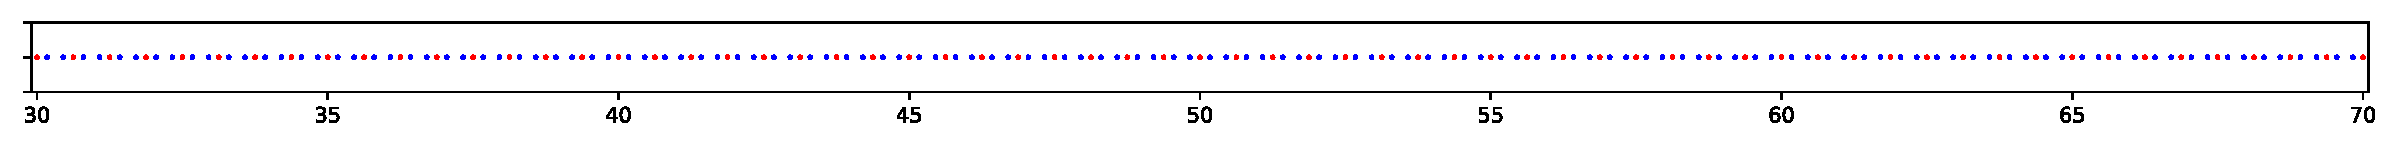
\includegraphics[scale=0.3]{ch3/node.pdf}
\end{center}
\begin{itemize}
        \item The number of spectral element, $N_h=64$
        \item The order of interpolation polynomial, $N_p=4$
\end{itemize}
Therefore, we now have $V$, a vector space  of dimension $193$. This vector space has a natural basis, or we called it the standard basis
\begin{equation}
        \{\textbf{e}_1, \textbf{e}_2, ..., \textbf{e}_{193}\}
\end{equation}
where
\begin{equation}
\textbf{e}_1=  \begin{bmatrix} 1 \\ 0 \\ \vdots \\ 0 \end{bmatrix}~~
\textbf{e}_2=  \begin{bmatrix} 0 \\ 1 \\ \vdots \\ 0 \end{bmatrix}~~
\cdots ~~
\textbf{e}_{193} = \begin{bmatrix} 0 \\ 0 \\ \vdots \\ 1 \end{bmatrix} 
\end{equation}

\section{Weight function, orthogonality and norm}
\begin{definition}[inner product]
By using integral calculus, it is common to use the following to define the inner product of two functions $f$ and $g$ with respect to a nonnegative weight function $w$ over an interval $[a, b]$:
\begin{equation}
        \langle f, g\rangle_w = \int_a^b f(x)g(x)w(x)\,dx \approx \sum_{i=1}^{193}w(x_i)f(x_i)g(x_i) 
\end{equation}
\end{definition}

\begin{definition}[weight function $w(x)$]
From the  Gauss-Lobatto quadrature, we have
\begin{center}
        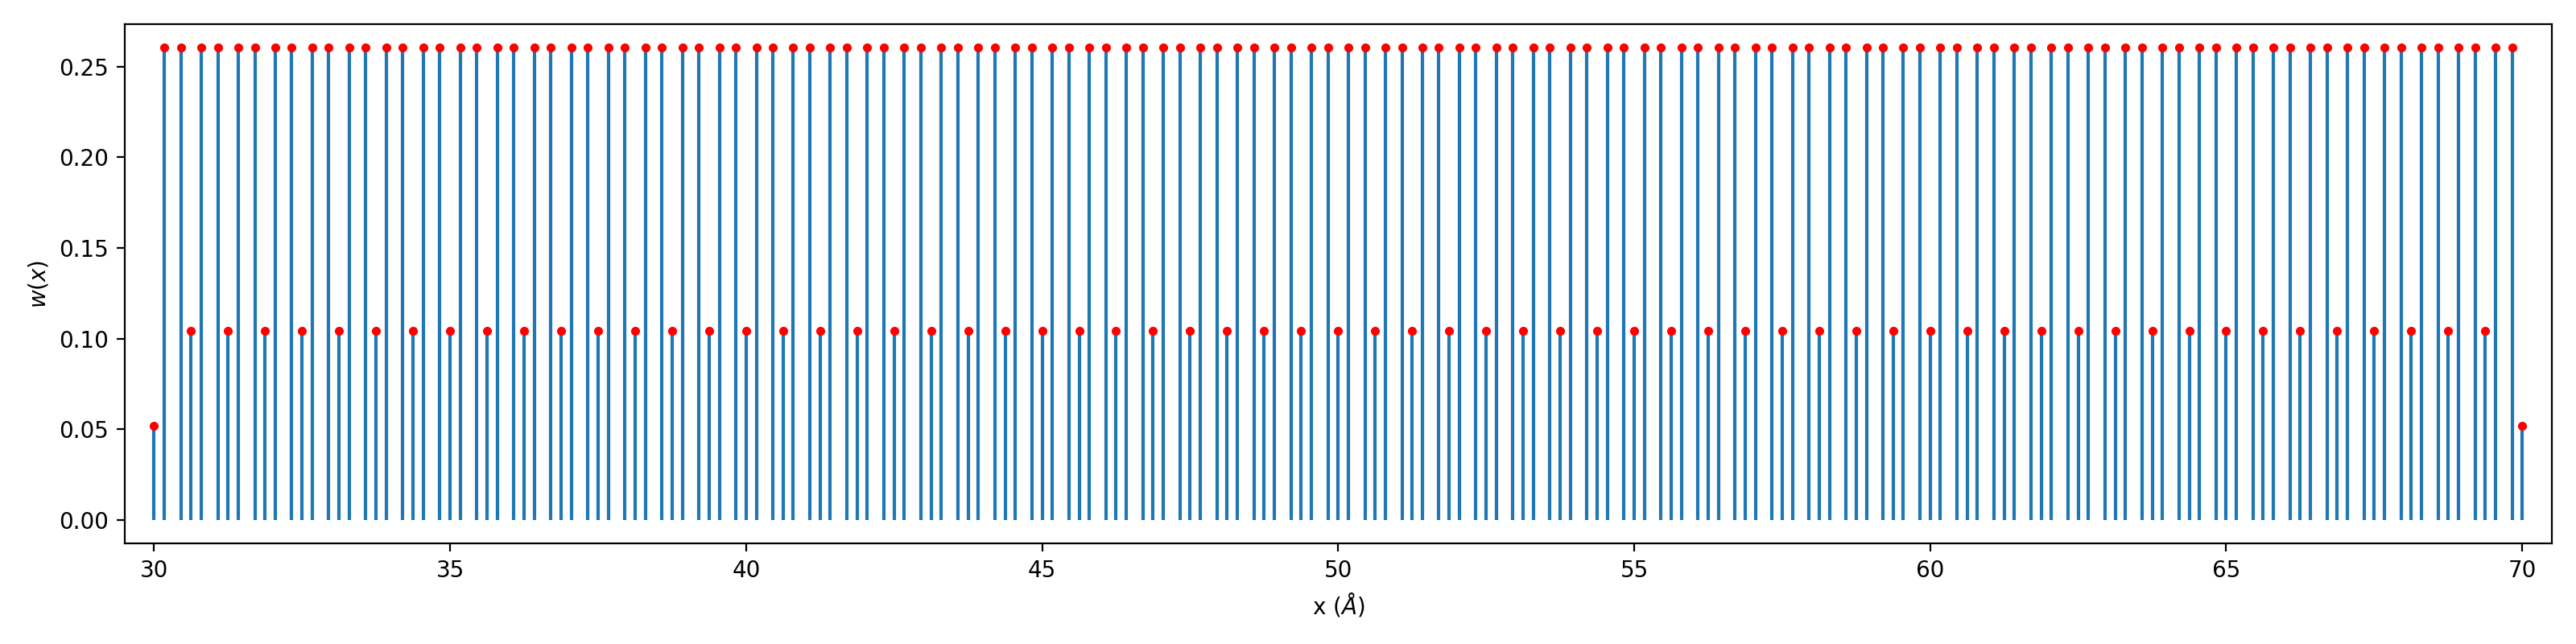
\includegraphics[scale=0.35]{ch3/weight_function.png}   
\end{center}
\end{definition}

\begin{definition}[Orthogonal]
We say that functions $f$ and $g$ are orthogonal if their inner product (equivalently, the value of this integral) is zero:
\begin{equation}
        \langle f,g\rangle _{w}=0.
\end{equation}
\end{definition}

\begin{definition}[Norm]
We define the norm with respect to this inner product as
\begin{equation}
        \|f\|_w = \sqrt{\langle f, f\rangle_w}
\end{equation}
\end{definition}

\section{Diagonalization of the operator}
\begin{definition}[Basis functions]
\begin{align}
        \psi^0_i(x) &= \rho_{\rm eq}(x) \phi^0_i(x) \\
        \phi^0_i(x) &= \sum_n c^0_n u_n(x).
\end{align}
\label{basisfunctions}
\end{definition}

\begin{definition}[Eigenvector matrix]
\begin{equation}
\Psi=
\begin{bmatrix}
\vert & \vert &  & \vert \\
\psi_1(x) & \psi_2(x) & \cdots & \psi_{N_v}(x) \\
\vert & \vert &  & \vert 
\end{bmatrix}
\end{equation}
\label{eigenvectormatrix}
Here, we get a set of orthonormal basis, $\langle \psi_i |$. The left part in the following part is 
\begin{equation}
        \Psi^T_{72\times 193}\Psi_{193 \times 72} = (\Psi^T\Psi)_{72 \times 72}
\end{equation}
The completeness relationship is actually can be seen by the blue points in the right part:
\begin{equation}
        \langle \psi_i(x),\psi_i(x)\rangle _{w} = \sum_{j=1}^{193}w(x_j)\psi_i(x_j)\psi_i(x_j)  = 1
\end{equation}
\begin{center}
        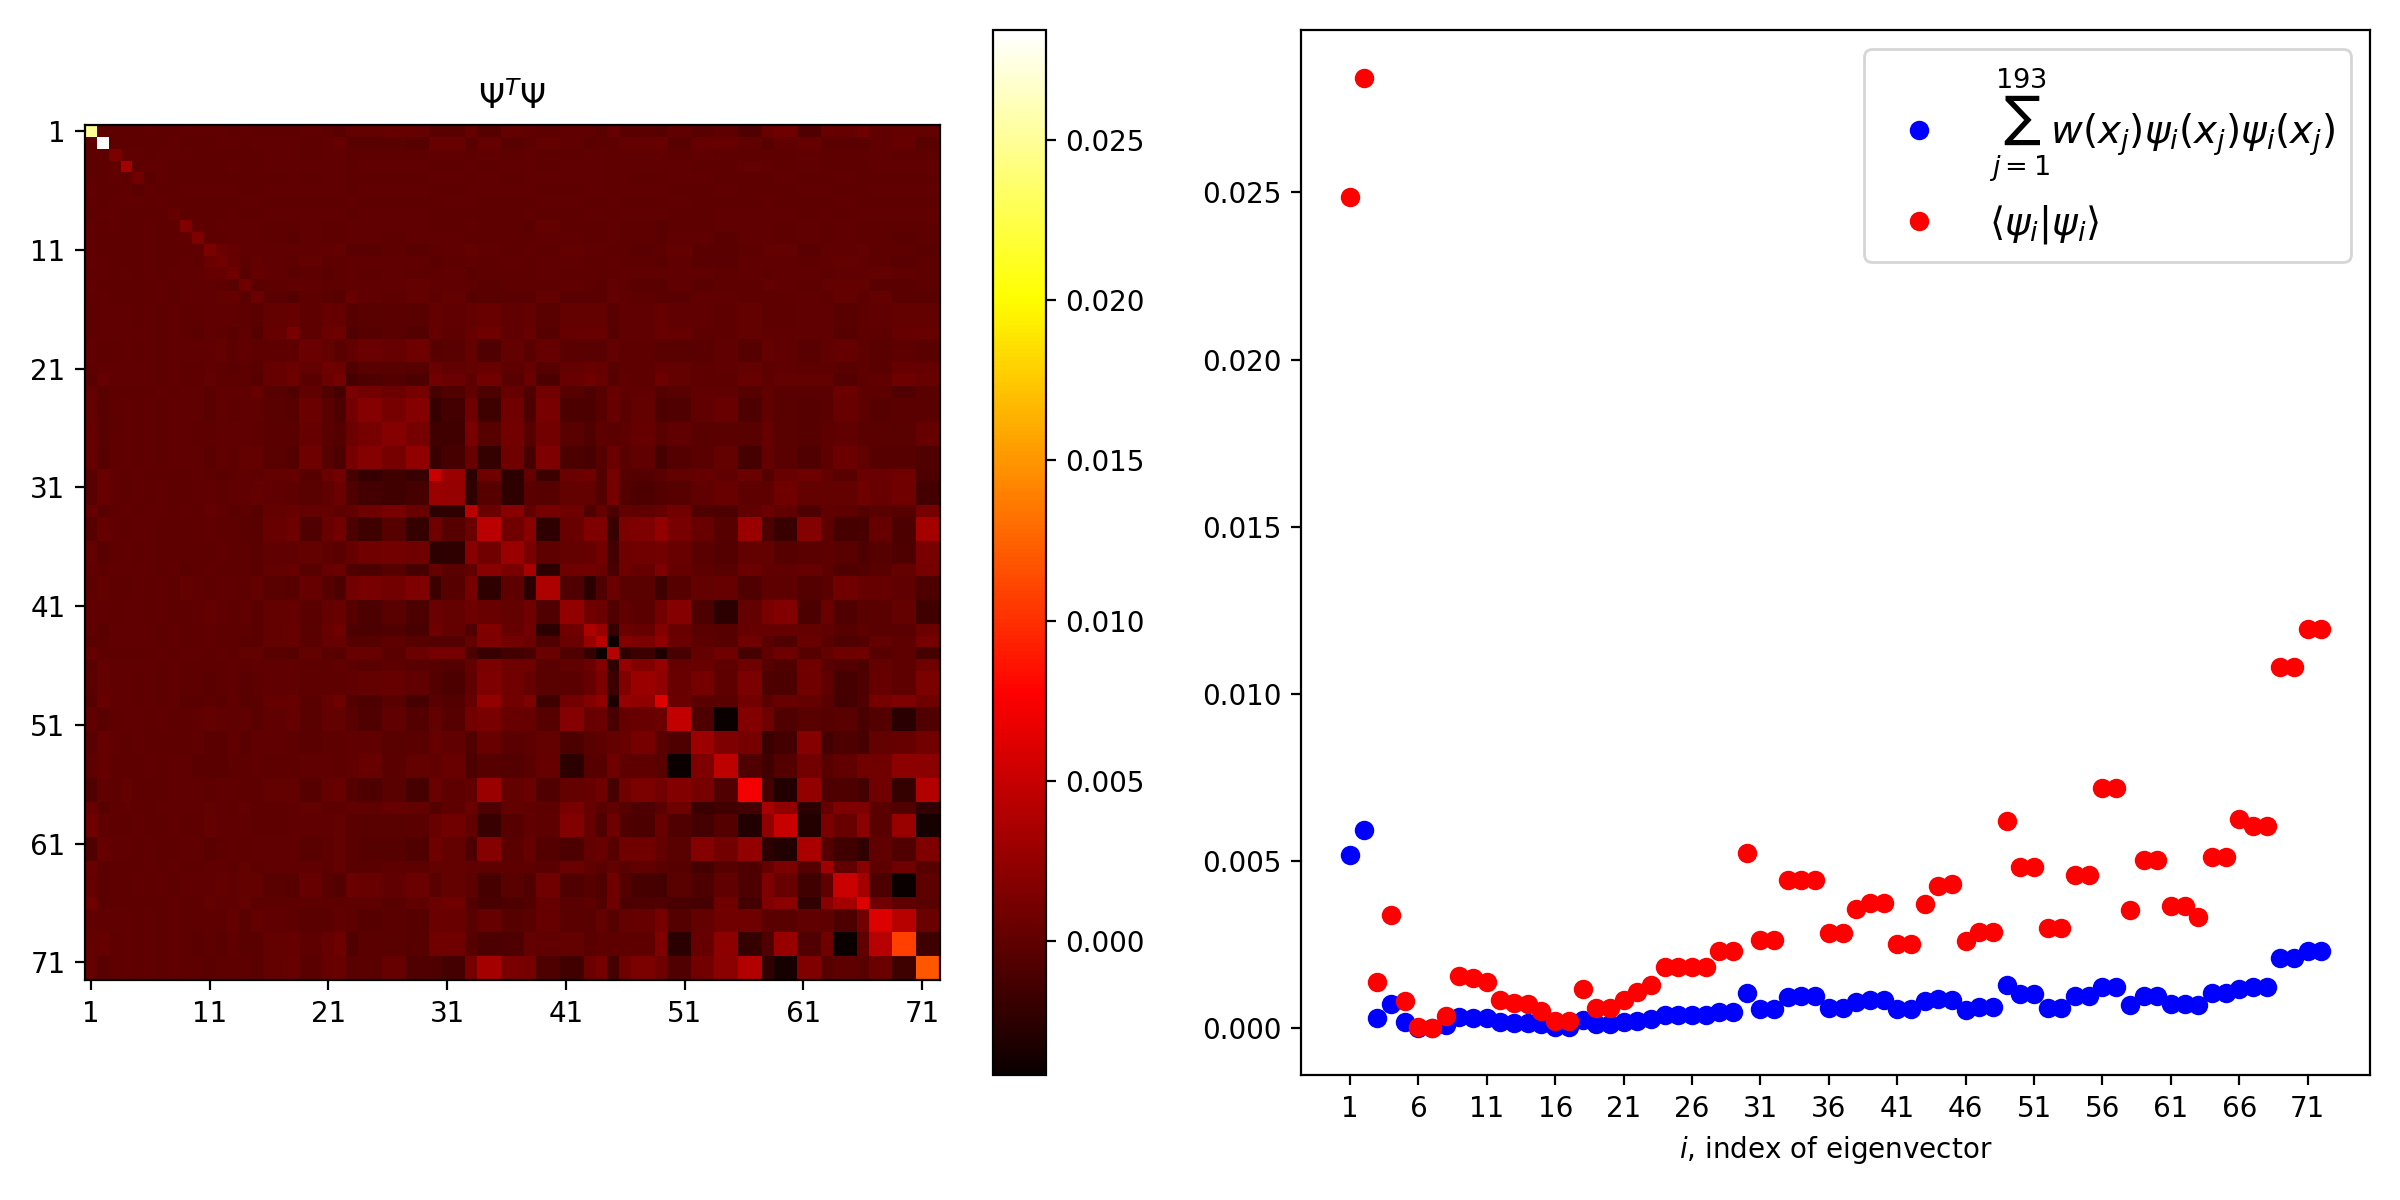
\includegraphics[scale=0.4]{ch3/eigenvec_matrix_complete.png}   
\end{center}
\end{definition}

